% !TeX root = main.tex
\section{UAV Design for Spraying Fertilizer}

The following are the given requirements

\begin{align*}
    \textup{Endurance} = 40 \, \textup{min} &&
    \textup{Range} = 5 \, \textup{Km} &&
    \textup{Payload weight} = 10 \, \textup{Kg} \\
    \textup{Flying altitude} = 20 \, \textup{m} &&
    \textup{Climb rate} = 1 \, \textup{m/s} &&
    \textup{Descent rate} = 2 \, \textup{m/s} \\
    \textup{Cruise speed} = 5 \, \textup{m/s}
\end{align*}

It is assumed that these are the minimum values and with a greater budget these can be extended.

% CONOPS
\subsection{CONOPS}

\textbf{CONOPS} or \emph{Concept of Operations} is the overview of the operations involved in the application of the UAV. The stages of operation are defined as

\begin{enumerate}
    \item \textbf{Takeoff} from ground and \textbf{climb} to an altitude of $20 \, m$. The climb rate is $1 \, m/s$.
    \item \textbf{Cruise} in straight lines while spraying fertilizer on the field. The equipment to carry out this operation is the payload (maximum $10 \, Kg$). The cruise speed is $5 \, m/s$. The UAV has the following modes of operation
    \begin{itemize}
        \item \emph{Manual control}: Giving the UAV velocity commands, directions, and manually controlling the fertilizer equipment.
        \item Calibrated \emph{autonomous control}: Calibrate the UAV to the field and configure the fertilizer distribution parameters. Then let the UAV perform the operation.
    \end{itemize}
    \item \textbf{Descent} after the task of spraying fertilizer is completed. Descent rate is $2 \, m/s$ from a height of $20 \, m$. After this, the UAV \textbf{lands}.
\end{enumerate}

% Requirements
\subsection{Requirement specifications}

The following can be considered the \emph{requirement specifications} for the starting of the design phase

\begin{itemize}
    \item \textit{Operating Velocity}: The cruise speed of the UAV is $5 \, m/s$.
    \item \textit{Range}: The total distance the UAV can travel without refuelling/recharging is $5 Km$.
    \item \textit{Endurance}: The total time the UAV can operate without refuelling/recharging is $40 \, min$.
    \item \textit{Payload}: The payload - fertilizer distribution unit and storage - is $10 \, Kg$ heavy.
    \item \textit{Wind} conditions: The UAV will be operated in wind speeds $4 \, km/hr$ to $9 \, km/hr$ \footnote{Weather data of Bangalore from \url{https://www.weatheronline.in} for Jan 2000 to Dec 2021, see wind speed and direction}. We can assume the \emph{upper limit of $10 \, km/hr$}. Most of the wind flows in the east and west direction.
    \item \textit{Altitude}: The flight altitude is capped at $20 \, m$ from ground. Must operate at a maximum of $1200\,m$ above sea level (ASL) to be used in most of agricultural India.
    \item \textit{Safety}: The UAV must be certified for safety standards in agriculture and UAV operations. It also must have regulatory compliance with GOI (Government of India) guidelines. The following can be noted \footnote{Main reference from \url{https://uavcoach.com/drone-laws-in-india/} and \url{https://digitalsky.dgca.gov.in/home}}
    \begin{itemize}
        \item The drone falls in the \emph{medium} category (weighing total of $25 \, kg$ to $150 \, kg$).
        \item Drone must have GPS, flight data logging, RTH (Return-to-home), anti-collision light, RFID and SIM with NPNT (No Permission No Takeoff) compliant software, and ID plate.
    \end{itemize}
    \item \textit{Maneuverability}: No agile maneuvers are needed. The drone will be oriented in the horizontal plane virtually always (no pitch and roll, only yaw).
\end{itemize}

% Market survey
\subsection{Market Survey}

\subsubsection*{DJI Agras T30}

The DJI Agras T30 UAV is a hexacopter (six propellers) suitable for agricultural applications. The main product can be found at \url{https://www.dji.com/t30}. Its specifications were obtained from \href{https://www.dji.com/t30/specs}{here}.

\begin{itemize}
    \item \textit{Operating Velocity}: The maximum operating velocity is $7\,m/s$, comfortably in the $5\,m/s$ bounds.
    \item \textit{Range}: The maximum range is around $7\,Km$ (calculated for operating at $6\,m/s$ for $20\,min$ which is comfortably in the operating bounds under $10\,Kg$ payload). However, the range of the remote control is $5\,Km$ to $7\,Km$.
    \item \textit{Endurance}: The maximum endurance of the drone is $20.5\,min$ on a single battery and the drone has provision for two batteries. Therefore, the total endurance it can get without charging is $41\,min$. This fits in our $40\,min$ requirement.
    \item \textit{Payload}: The maximum payload is $40\,Kg$, which is beyond our requirement of only $10\,Kg$
    \item \textit{Wind conditions}: It can operate at wind speeds of up to $8\,m/s$ (or $28.8\,Km/hr$). Our requirement is just $10\,Km/hr$.
    \item \textit{Altitude}: The maximum flight altitude is $4500\,m$. This is well beyond our requirement of $1200\,m$.
    \item \textit{Safety}: The UAV has RTH (return-to-home) built-in. Regulatory compliance by GOI will require extra software setup, but it possible.
\end{itemize}

With the above specifications, the UAV almost exceeds our requirements. Choosing it should give very comfortable bounds, thereby allowing for greater needs in the future.
However, the price would be around \rupee~700,000. This drone is shown in figure \ref{fig:sfig-q1-ms-dji}.

\subsubsection*{FAE 1115 Octa - Predator}

The FAE 1115 Octa Predator is an octacopter (eight propellers) suitable for carrying heavy payloads for agricultural applications. The product can be found at \href{https://fae-drones.com/products/FAE-1115-Octa-PREDATOR-40.html}{fae-drones.com}. Its specifications are as follows

\begin{itemize}
    \item \textit{Operating velocity}: The mentioned maximum speed is $80\,Km/hr \approx 22\,m/s$. This is much more than our required $5\,m/s$.
    \item \textit{Range}: The range is mentioned as $20\,Km$. This is much more than our desired $5\,Km$.
    \item \textit{Endurance}: The flight time is mentioned as $40\,min$ which exactly meets our requirements. However, this reduces to $20\,min$ if the payload increases beyond $10\,Kg$.
    \item \textit{Payload}: The recommended payload is around $5\,Kg$, but the maximum is $10\,Kg$ with reduced flight time.
    \item \textit{Wind conditions}: The UAV can operate in wind conditions of up to $50\,Km/hr \approx 13.8\,m/s$. This is within our requirement of $10\,Km/hr$.
    \item \textit{Altitude}: The maximum flight altitude is $3500\,m$ which is more than our required $1200\,m$.
    \item \textit{Safety}: The UAV has RTH functionality and will require software modifications to make it compliant with GOI norms.
\end{itemize}

The UAV above fits our requirements by a narrow margin (even cutting it short sometimes). The price would be around \rupee~500,000. This drone is shown in figure \ref{fig:sfig-q1-ms-fae}.

\subsection*{DroneStark Octaglide}

The DroneStark Octaglide UAV is a versatile dual quadcopter UAV (eight propellers arranged in the quadcopter configuration - also called \emph{X8} configuration). The main product can be found \href{https://www.dronestark.com/octaglide}{here}. Its specifications are as follows 
\footnote{Obtained from \url{https://www.dronestark.com/octaglide} and \url{https://www.dronestark.com/flying-beyond-limits}}

\begin{itemize}
    \item \textit{Operating Velocity}: The mentioned maximum speed of the drone is $20\,m/s$. This is much more than our required $5\,m/s$
    \item \textit{Range}: The range is mentioned as $9\,Km$ during testing. This is above our requirement of $5\,Km$.
    \item \textit{Endurance}: The flight time is mentioned as $24\,min$ with a $60,000\,mAh$ battery. Extra batteries can be added on board, using which this can be increases to match with our requirement of $40\,min$.
    \item \textit{Payload}: The drone can carry payloads of upto $20\,Kg$. This is much more than our requirement of $10\,Kg$ payload.
    \item \textit{Wind conditions}: The UAV can operate in wind conditions of $12\,m/s \approx 43.2\,Km/hr$. This is more than our requirement of $10\,Km/hr$.
    \item \textit{Altitude}: The UAV can operate at altitudes of $5000\,m$ above sea level with a payload of $10\,Kg$ (it is $3500\,m$ with $20\,Kg$ payload). This is more than our requirement of $1200\,m$.
    \item \textit{Safety}: The drone has BVLOS (Beyond Visual Line of Sight) RTH (return to home) even \emph{without} radio link or communication. It is compliant with all GOI norms out-of-box as it is manufactured in India.
\end{itemize}

The UAV fits in our requirement bounds (with very little augmentation out of the box). Unfortunately, a price quote could not be found online, but since it does not have any customs attached, it will probably be the cheapest option (as it is \emph{made in India}). This drone is shown in figure \ref{fig:sfig-q1-ms-ds}.

\begin{figure}[t]
    \centering
    % DJI Agras T30
    \begin{subfigure}[b]{0.3\textwidth}
        \centering
        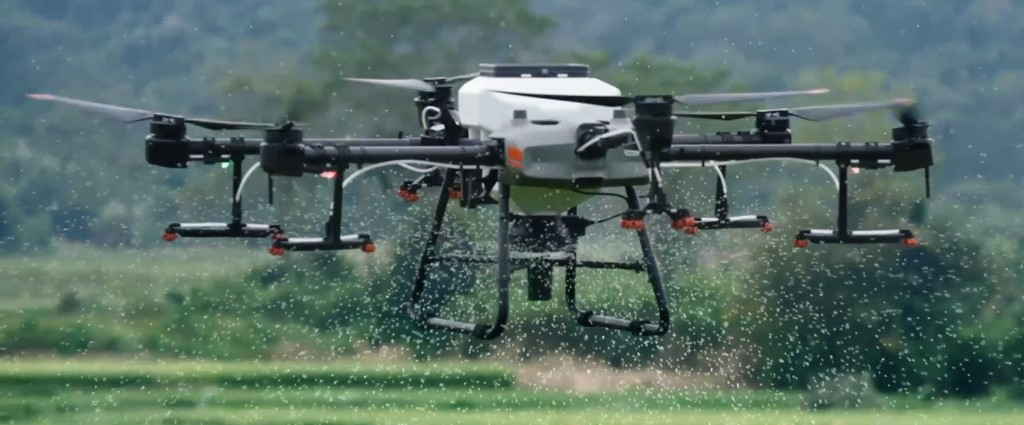
\includegraphics[width=\textwidth]{DJI-Agras-T30.jpg}
        \caption{DJI Agras T30}
        \label{fig:sfig-q1-ms-dji}
    \end{subfigure}
    % FAE 1115 Octa - Predator
    \begin{subfigure}[b]{0.3\textwidth}
        \centering
        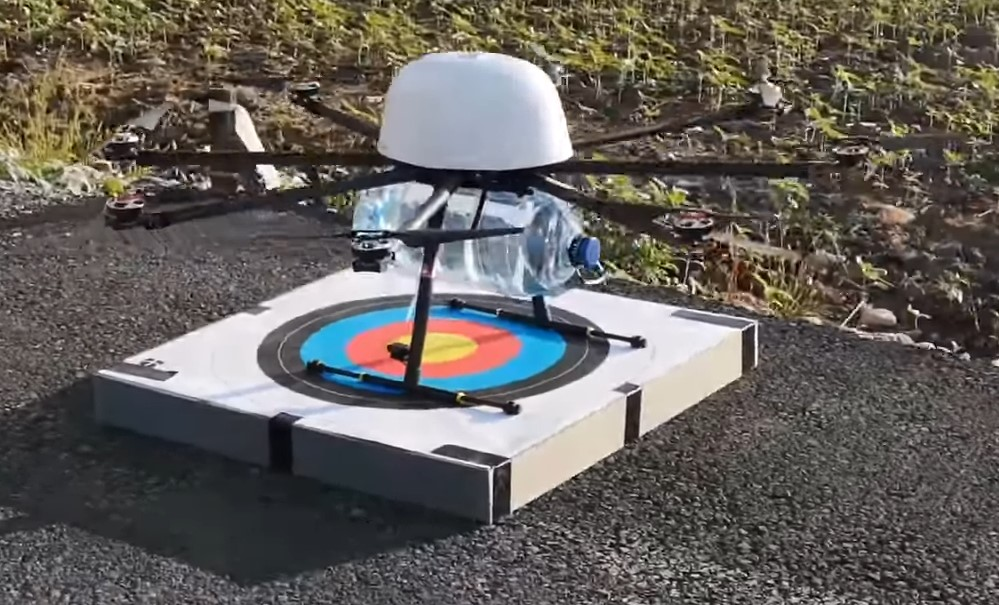
\includegraphics[width=\textwidth]{FAE-1115-Octa-Predator.jpg}
        \caption{FAE 1115 Octa - Predator}
        \label{fig:sfig-q1-ms-fae}
    \end{subfigure}
    % DroneStark Octaglide
    \begin{subfigure}[b]{0.3\textwidth}
        \centering
        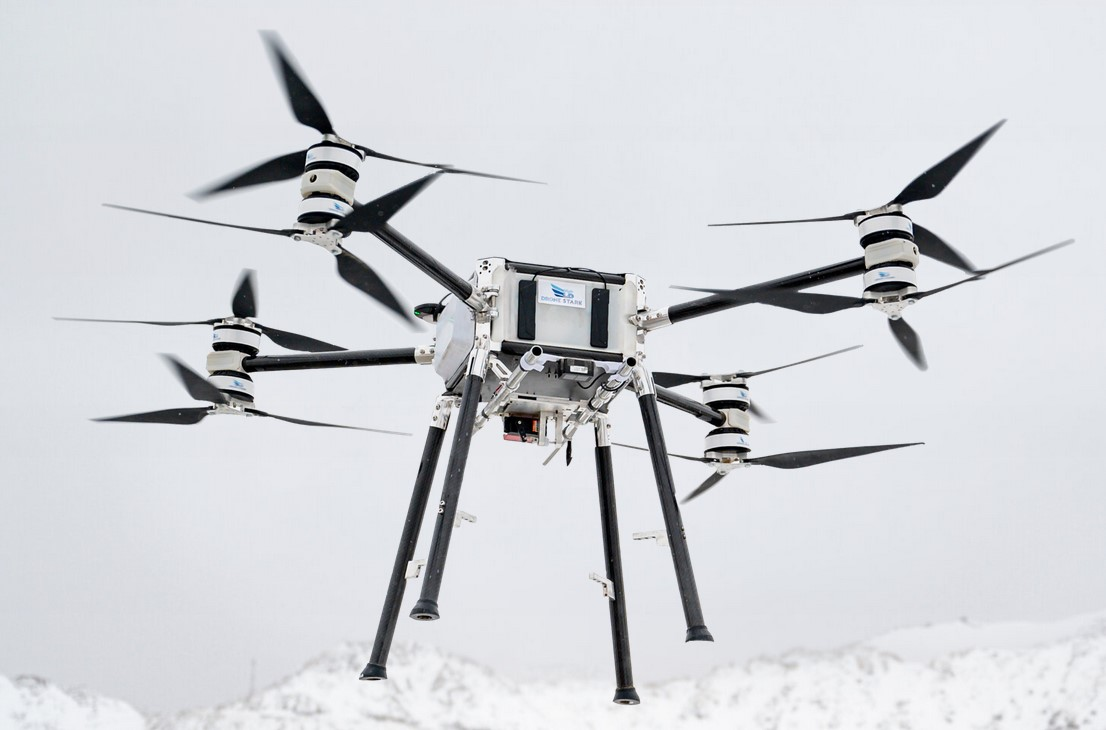
\includegraphics[width=\textwidth]{DroneStark-Octaglide.jpg}
        \caption{FAE 1115 Octa - Predator}
        \label{fig:sfig-q1-ms-ds}
    \end{subfigure}
    \caption{UAVs identified in market survey}
    \label{fig:q1-market-survey}
    \small
        Figure \ref{sub@fig:sfig-q1-ms-dji} is from \url{https://www.dji.com/t30}, figure \ref{sub@fig:sfig-q1-ms-fae} is from \url{https://youtu.be/7wkKQ1ad528}, and figure \ref{sub@fig:sfig-q1-ms-ds} is from \url{https://www.dronestark.com/}
\end{figure}

